\documentclass[11pt]{article}

\usepackage[margin=1in]{geometry}
\usepackage{amsmath,amssymb,mathtools}
\usepackage{booktabs,array}
\usepackage{hyperref}
\usepackage{xcolor}
\usepackage{microtype}
\usepackage{fancyhdr}
\usepackage{float}
\usepackage{tikz}
\usetikzlibrary{arrows.meta}

\definecolor{linkblue}{RGB}{25,74,130}
\definecolor{softblue}{RGB}{237,244,251}
\definecolor{softgray}{RGB}{246,246,246}
\hypersetup{
  colorlinks=true,
  linkcolor=linkblue,
  urlcolor=linkblue,
  citecolor=linkblue,
  pdftitle={Three-qubit, two-cavity Hamiltonian},
  pdfauthor={qumode sep technical note}
}

\pagestyle{fancy}
\fancyhf{}
\lhead{3 qubits + 2 cavities}
\rhead{\thepage}
\setlength{\headheight}{14pt}

\newcommand{\Pe}[1]{\lvert e\rangle\!\langle e\rvert_{#1}}
\newcommand{\Ujp}{\hat{U}_{\mathrm{JP}}}
\newcommand{\Pab}{\hat{\Pi}_{AB}}

\title{\textbf{The 3-qubit, 2-cavity Hamiltonian}\\
\large Matched $\chi_{qA}=\chi_{qB}$ JP gate and unitless Lindblad rates}
\author{\texorpdfstring{\texttt{qumode\_sep}}{qumode sep} technical note}
\date{\today}

\begin{document}
\maketitle

\begin{abstract}
Laboratory Hamiltonian of two storage cavities $A,B$ and three transmons
$d,q,e$; conversion of device frequencies into the unitless rates used by a
Lindblad solver; and the joint-parity (JP) gate as a finite-time evolution
under a matched shared dispersive coupling.
\end{abstract}

\section{Hardware}

Five modes in a chain $d$--$A$--$q$--$B$--$e$ (Fig.~\ref{fig:hardware}).
Cavities $A,B$ are the qumodes.  Transmons $d,e$ are local ECD ancillas.
Transmon $q$ is the shared coupler.  This is the two-cavity extension of the
one-qumode device in Dutta \emph{et al.}\ \cite{Dutta2025} and the Alice/Bob
layout of Gao \emph{et al.}\ \cite{Gao2018}.

\begin{figure}[H]
\centering
\resizebox{\textwidth}{!}{%
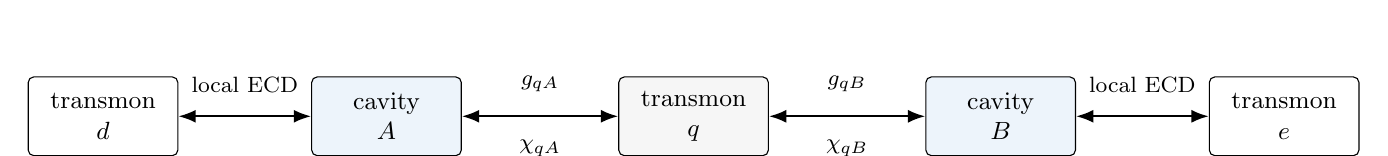
\begin{tikzpicture}[
  box/.style={draw, rounded corners=2pt, minimum width=1.9cm,
              minimum height=1.0cm, align=center, font=\small, inner sep=3pt},
  both/.style={{Latex[length=2.2mm]}-{Latex[length=2.2mm]}, thick},
  note/.style={font=\footnotesize, align=center}
]
  \node[box] (d) at (0,0) {transmon\\$d$};
  \node[box, fill=softblue] (a) at (3.6,0) {cavity\\$A$};
  \node[box, fill=softgray] (q) at (7.5,0) {transmon\\$q$};
  \node[box, fill=softblue] (b) at (11.4,0) {cavity\\$B$};
  \node[box] (e) at (15.0,0) {transmon\\$e$};
  \draw[both] (d) -- node[above=5pt,note] {local ECD} (a);
  \draw[both] (a) --
    node[above=5pt,note] {$g_{qA}$}
    node[below=5pt,note] {$\chi_{qA}$} (q);
  \draw[both] (q) --
    node[above=5pt,note] {$g_{qB}$}
    node[below=5pt,note] {$\chi_{qB}$} (b);
  \draw[both] (b) -- node[above=5pt,note] {local ECD} (e);
\end{tikzpicture}%
}
\caption{Three transmons and two cavities.  For a single-wait JP we set
$\chi_{qA}=\chi_{qB}$.}
\label{fig:hardware}
\end{figure}

\section{Laboratory Hamiltonian}

Let $\hat{a}$ ($\hat{b}$) annihilate a photon in $A$ ($B$), and let
$\hat{c}_d,\hat{c}_q,\hat{c}_e$ lower the transmons.  Rotating-wave form:
\begin{align}
\frac{\hat{H}}{\hbar}
&=\omega_A\hat{a}^\dagger\hat{a}+\omega_B\hat{b}^\dagger\hat{b}
 +\sum_{j\in\{d,q,e\}}
  \Bigl[\omega_j\hat{c}_j^\dagger\hat{c}_j
        +\tfrac{\alpha_j}{2}\hat{c}_j^\dagger\hat{c}_j
         (\hat{c}_j^\dagger\hat{c}_j-1)\Bigr]
\nonumber\\
&\quad
 +g_{dA}(\hat{a}^\dagger\hat{c}_d+\hat{a}\hat{c}_d^\dagger)
 +g_{eB}(\hat{b}^\dagger\hat{c}_e+\hat{b}\hat{c}_e^\dagger)
\nonumber\\
&\quad
 +g_{qA}(\hat{a}^\dagger\hat{c}_q+\hat{a}\hat{c}_q^\dagger)
 +g_{qB}(\hat{b}^\dagger\hat{c}_q+\hat{b}\hat{c}_q^\dagger)
 +\hat{H}_{\mathrm{drive}}(t)/\hbar .
\label{eq:lab}
\end{align}
Direct $d$--$B$, $e$--$A$, and $d$--$e$ couplings are dropped.  Cavities are
detuned by $\sim 1~\mathrm{GHz}$ so they do not hybridize \cite{Gao2018}.

Far off resonance, $\Delta_{j\mu}=\omega_j-\omega_\mu$, each transmon--cavity
pair has a dispersive shift
$\chi_{j\mu}=g_{j\mu}^2\alpha_j/[\Delta_{j\mu}(\Delta_{j\mu}+\alpha_j)]$.

In the lab, $\chi_{qA}$ is a measured frequency difference, not a derived
symbol.  Probe cavity $A$ with a weak tone: the resonance peak sits at one
frequency when $q$ is in $\lvert g\rangle$ and at another when $q$ is in
$\lvert e\rangle$.  That peak-to-peak gap is $\chi_{qA}/2\pi$ (typically
quoted in $\mathrm{MHz}$).  Equivalently, park a photon in $A$ and
spectroscopy $q$: the transmon line splits into a ladder
$\omega_q,\ \omega_q-\chi_{qA},\ \omega_q-2\chi_{qA},\ldots$ indexed by
photon number $n_A$ (number splitting).  Either way, what moved is a
resonance you read on a network analyzer or a qubit spectroscopy scan.
The same measurement on $q$--$B$, $d$--$A$, and $e$--$B$ gives
$\chi_{qB}$, $\chi_{dA}$, and $\chi_{eB}$.
\begin{align}
\frac{\hat{H}_{\mathrm{disp}}}{\hbar}
&=\widetilde\omega_A\hat{n}_A+\widetilde\omega_B\hat{n}_B
 +\sum_{j\in\{d,q,e\}}\widetilde\omega_j\Pe{j}
\nonumber\\
&\quad
 -\chi_{dA}\,\hat{n}_A\Pe{d}
 -\chi_{eB}\,\hat{n}_B\Pe{e}
 -\chi_{qA}\,\hat{n}_A\Pe{q}
 -\chi_{qB}\,\hat{n}_B\Pe{q}
\nonumber\\
&\quad
 -\tfrac{K_A}{2}\hat{n}_A(\hat{n}_A-1)
 -\tfrac{K_B}{2}\hat{n}_B(\hat{n}_B-1)
 -K_{AB}\hat{n}_A\hat{n}_B ,
\label{eq:disp}
\end{align}
with $\hat{n}_A=\hat{a}^\dagger\hat{a}$, $\hat{n}_B=\hat{b}^\dagger\hat{b}$.
The $\widetilde\omega$ are Lamb-shifted bare frequencies.  They imprint
ordinary dynamical phases $e^{-i\widetilde\omega_A n\tau}$ on Fock states;
Kerr imprints extra $n$-dependent phases.  Both are kept in the Lindblad
generator below.

\paragraph{Matched shared coupling.}
JP is a wait under $-\chi_{qA}\hat{n}_A\Pe{q}-\chi_{qB}\hat{n}_B\Pe{q}$.
One wait of duration $\tau$ maps joint parity onto $q$ iff
$\chi_{qA}\tau$ and $\chi_{qB}\tau$ are both odd multiples of $\pi$.
The easy choice is to set them equal,
\begin{equation}
\chi_{qA}=\chi_{qB},\qquad \tau=\pi/\chi_{qA} .
\label{eq:match}
\end{equation}
No extra symbol is needed: after this identification the shared term is
$-\chi_{qA}(\hat{n}_A+\hat{n}_B)\Pe{q}$.
Because $\omega_A\neq\omega_B$, equal $\chi_{qA}=\chi_{qB}$ generally means
\emph{unequal} $g_{qA},g_{qB}$.  Unmatched shared shifts (Wang:
$0.71$ vs $1.41~\mathrm{MHz}$ \cite{Wang2016}) need two different waits;
we do not use that here.

The local shifts $\chi_{dA}$ and $\chi_{eB}$ are \emph{not} used by JP.
They set the ECD rate on $(d,A)$ and $(e,B)$ and may be chosen
independently of $\chi_{qA}$ and of each other (Eickbusch ECD:
$\chi_{dA}/2\pi=33~\mathrm{kHz}$ while $\chi_{qA}/2\pi\sim 1~\mathrm{MHz}$).
They still act during the JP wait as spectators
$-\chi_{dA}\hat{n}_A\Pe{d}-\chi_{eB}\hat{n}_B\Pe{e}$.  If
$d$ or $e$ is in superposition those terms add extra phases; echo
$X_d X_e$ at the midpoint, or leave them in the Lindblad Hamiltonian
and accept the error.

\section{From SI frequencies to unitless numbers}

A Lindblad solver takes $\hbar=1$ and a Hamiltonian whose eigenvalues are
inverse times.  Pick one laboratory rate as the unit.  Here that unit is
the matched shared shift $\chi_{qA}$ (with $\chi_{qA}=\chi_{qB}$, so
$\chi_{qA}=1$ in code).

\textit{Recipe.}  For every laboratory angular frequency $\Omega$
(already in $\mathrm{rad/s}$, i.e.\ $2\pi$ times the quoted $\mathrm{Hz}$),
store
\begin{equation}
\widetilde{\Omega}=\Omega/\chi_{qA} .
\end{equation}
Laboratory time $t$ becomes $\tilde t=\chi_{qA} t$.  Jump rates follow the
same rule: $\tilde\kappa=\kappa/\chi_{qA}$.  Dimensionless noise over a
gate of duration $\tau$ is the product $\kappa\tau=\tilde\kappa\,\tilde\tau$,
which is the parameter used by Dutta \emph{et al.}\ \cite{Dutta2025}.

From Eickbusch \cite{Eickbusch2022} and Wang \cite{Wang2016}:
\begin{center}
\small
\renewcommand{\arraystretch}{1.2}
\begin{tabular}{lccc}
\toprule
quantity & laboratory & unit $\chi_{qA}/2\pi=1~\mathrm{MHz}$ & notes\\
\midrule
$\chi_{qA}=\chi_{qB}$
  & $1~\mathrm{MHz}$ (choose matched)
  & $1$
  & time unit $1/\chi_{qA}\approx 0.16~\mathrm{\mu s}$\\
$\chi_{dA}=\chi_{eB}$
  & $33~\mathrm{kHz}$ \cite{Eickbusch2022}
  & $0.033$
  & local ECD, kept weak\\
$\kappa_A=\kappa_B=1/T_{1,\mathrm{cav}}$
  & $T_{1,\mathrm{cav}}=436~\mathrm{\mu s}$
  & $\tilde\kappa=3.65\times10^{-4}$
  & $\kappa/2\pi\simeq365~\mathrm{Hz}$ \cite{Dutta2025}\\
$\gamma_q=1/T_{1,q}$
  & $T_{1,q}\approx50~\mathrm{\mu s}$
  & $\tilde\gamma_q=3.18\times10^{-3}$
  & transmon relaxation\\
$\gamma_{\phi,q}$ from $T_{2}\approx30~\mathrm{\mu s}$
  & $T_{2}^{-1}-T_{1}^{-1}/2$
  & $\tilde\gamma_{\phi,q}\approx1.8\times10^{-3}$
  & extra dephasing of $q$\\
\bottomrule
\end{tabular}
\end{center}
Conversion of the cavity row, written out:
\begin{equation}
\chi_{qA}=2\pi\times10^{6}~\mathrm{s}^{-1},\quad
\kappa=\frac{1}{436~\mathrm{\mu s}}\simeq2.29\times10^{3}~\mathrm{s}^{-1},\quad
\tilde\kappa=\frac{\kappa}{\chi_{qA}}=3.65\times10^{-4}.
\end{equation}
A wait $\tau=\pi/\chi_{qA}$ then has $\kappa\tau=\pi\tilde\kappa\simeq1.15\times10^{-3}$,
the same $10^{-3}$ scale as the per-ECD-block $\kappa\tau\sim1.5\times10^{-3}$
in Ref.~\cite{Dutta2025}.

\section{JP gate}

The joint-parity operator on the two cavities is
\begin{equation}
\Pab
=(-1)^{\hat{n}_A+\hat{n}_B}
=\hat{\Pi}_A\hat{\Pi}_B,
\qquad
\hat{\Pi}_A=(-1)^{\hat{n}_A},\quad
\hat{\Pi}_B=(-1)^{\hat{n}_B}.
\end{equation}
It is diagonal in the Fock basis.  On a product number state
$\lvert n,m\rangle\equiv\lvert n\rangle_A\otimes\lvert m\rangle_B$,
\begin{equation}
\Pab\lvert n,m\rangle
=(-1)^{n+m}\lvert n,m\rangle
=
\begin{cases}
+\lvert n,m\rangle & n+m\text{ even},\\
-\lvert n,m\rangle & n+m\text{ odd}.
\end{cases}
\end{equation}
Equivalently, the four parity sectors are
\begin{center}
\small
\begin{tabular}{cccc}
\toprule
parity of $n$ & parity of $m$ & $n+m$ & $\Pab$ eigenvalue\\
\midrule
even & even & even & $+1$\\
even & odd  & odd  & $-1$\\
odd  & even & odd  & $-1$\\
odd  & odd  & even & $+1$\\
\bottomrule
\end{tabular}
\end{center}
The odd-joint-parity projector is the $+1$ eigenspace of
$(\hat{\mathbb{I}}-\Pab)/2$:
\begin{equation}
\hat{P}_{\mathrm{odd}}
=\frac{\hat{\mathbb{I}}-\Pab}{2},\qquad
\hat{P}_{\mathrm{odd}}\lvert n,m\rangle
=
\begin{cases}
0 & n+m\text{ even},\\
\lvert n,m\rangle & n+m\text{ odd}.
\end{cases}
\end{equation}
The JP gate is a $\pi/2$ phase on that subspace,
\begin{equation}
\boxed{
\Ujp
=\exp\!\bigl[-i(\pi/2)\hat{P}_{\mathrm{odd}}\bigr]
=e^{-i\pi/4}\exp\!\bigl[+i(\pi/4)\Pab\bigr],
}
\label{eq:jp}
\end{equation}
so
\begin{equation}
\Ujp\lvert n,m\rangle
=(-i)^{(n+m)\bmod 2}\lvert n,m\rangle
=
\begin{cases}
+\lvert n,m\rangle & n+m\text{ even},\\
-i\lvert n,m\rangle & n+m\text{ odd}.
\end{cases}
\end{equation}

\paragraph{Time evolution that realizes it.}
Initialize $q$ in $\lvert g\rangle$.  With $\chi_{qA}=\chi_{qB}$ the shared
term in Eq.~\eqref{eq:disp} is
$\hat{H}_{\mathrm{JP}}/\hbar=-\chi_{qA}(\hat{n}_A+\hat{n}_B)\Pe{q}$.
In unitless time ($\chi_{qA}=1$),
$\hat{\widetilde{H}}_{\mathrm{JP}}=-(\hat{n}_A+\hat{n}_B)\Pe{q}$, so a wait
$\tilde\tau=\pi$ is
\begin{equation}
\hat{U}_\pi
=\lvert g\rangle\!\langle g\rvert_q
 +\lvert e\rangle\!\langle e\rvert_q\,\Pab :
\quad
\hat{U}_\pi\lvert g,n,m\rangle=\lvert g,n,m\rangle,\quad
\hat{U}_\pi\lvert e,n,m\rangle=(-1)^{n+m}\lvert e,n,m\rangle.
\end{equation}
Qubit rotations are
$R_y(\pi/2)\lvert g\rangle=(\lvert g\rangle+\lvert e\rangle)/\sqrt{2}$
and
$R_y(-\pi/2)(\lvert g\rangle\pm\lvert e\rangle)/\sqrt{2}=\lvert g\rangle$
or $\lvert e\rangle$ (even/odd superposition).  Virtual
$S^\dagger\lvert g\rangle=\lvert g\rangle$,
$S^\dagger\lvert e\rangle=-i\lvert e\rangle$.
Write $\lambda=(-1)^{n+m}$ and start from $\lvert g,n,m\rangle$.

\textit{Even} ($n+m$ even, $\lambda=+1$):
\begin{align*}
R_y(+\pi/2)
  &\colon\ (\lvert g\rangle+\lvert e\rangle)/\sqrt{2}\,\lvert n,m\rangle\\
\hat{U}_\pi
  &\colon\ (\lvert g\rangle+\lvert e\rangle)/\sqrt{2}\,\lvert n,m\rangle
  \quad\text{(no relative phase)}\\
R_y(-\pi/2)
  &\colon\ \lvert g,n,m\rangle\\
S^\dagger
  &\colon\ \lvert g,n,m\rangle\\
R_y(+\pi/2),\ \hat{U}_\pi,\ R_y(-\pi/2)
  &\colon\ \lvert g,n,m\rangle.
\end{align*}
Net: $+\lvert n,m\rangle$, $q$ back in $\lvert g\rangle$.

\textit{Odd} ($n+m$ odd, $\lambda=-1$):
\begin{align*}
R_y(+\pi/2)
  &\colon\ (\lvert g\rangle+\lvert e\rangle)/\sqrt{2}\,\lvert n,m\rangle\\
\hat{U}_\pi
  &\colon\ (\lvert g\rangle-\lvert e\rangle)/\sqrt{2}\,\lvert n,m\rangle\\
R_y(-\pi/2)
  &\colon\ -\lvert e,n,m\rangle
  \quad\text{(parity now stored on $q$)}\\
S^\dagger
  &\colon\ i\lvert e,n,m\rangle
  \quad\text{($-i$ on $\lvert e\rangle$ times the minus sign)}\\
R_y(+\pi/2)
  &\colon\ i(-\lvert g\rangle+\lvert e\rangle)/\sqrt{2}\,\lvert n,m\rangle\\
\hat{U}_\pi
  &\colon\ i(-\lvert g\rangle-\lvert e\rangle)/\sqrt{2}\,\lvert n,m\rangle\\
R_y(-\pi/2)
  &\colon\ -i\lvert g,n,m\rangle.
\end{align*}
Net: $-i\lvert n,m\rangle$, $q$ back in $\lvert g\rangle$.

Together this is $\lvert g\rangle\otimes\Ujp\lvert n,m\rangle$.  Local $d,e$
are spectators (echo them if $\chi_{dA},\chi_{eB}$ must not act).

\paragraph{Duration.}
Idle time is two waits of $\pi/\chi_{qA}$.  With
$\chi_{qA}/2\pi=1~\mathrm{MHz}$,
\begin{equation}
\tau_{\mathrm{JP}}=\frac{2\pi}{\chi_{qA}}=1~\mathrm{\mu s}
\qquad\bigl(\tilde\tau_{\mathrm{JP}}=2\pi\text{ in code}\bigr).
\end{equation}
Four transmon $\pi/2$ pulses add $\sim 100~\mathrm{ns}$
($t_q=24~\mathrm{ns}$ \cite{Eickbusch2022}) and can be treated as
instantaneous relative to the waits.

\paragraph{Lindblad equation during the waits
(unitless, $\chi_{qA}=\chi_{qB}=1$).}
Use the \emph{full} 3-qubit, 2-cavity Hamiltonian Eq.~\eqref{eq:disp} so
every Fock- and transmon-dependent phase is present:
\begin{align}
\hat{\widetilde{H}}
=\frac{\hat{H}_{\mathrm{disp}}}{\hbar\chi_{qA}}
&=\tilde\omega_A\hat{n}_A+\tilde\omega_B\hat{n}_B
 +\sum_{j\in\{d,q,e\}}\tilde\omega_j\Pe{j}
\nonumber\\
&\quad
 -\tilde\chi_{dA}\,\hat{n}_A\Pe{d}
 -\tilde\chi_{eB}\,\hat{n}_B\Pe{e}
 -(\hat{n}_A+\hat{n}_B)\Pe{q}
\nonumber\\
&\quad
 -\tfrac{\tilde K_A}{2}\hat{n}_A(\hat{n}_A-1)
 -\tfrac{\tilde K_B}{2}\hat{n}_B(\hat{n}_B-1)
 -\tilde K_{AB}\hat{n}_A\hat{n}_B ,
\label{eq:Htilde}
\end{align}
with $\tilde\chi_{dA}=\tilde\chi_{eB}=0.033$ and
$\tilde K\sim10^{-3}$--$10^{-2}$ ($K/2\pi\sim1$--$10~\mathrm{kHz}$
\cite{Wang2016}).  The $\tilde\omega$ rows are the free phases
($\tilde\omega_A=\widetilde\omega_A/\chi_{qA}\simeq5260$ if the cavity is at
$5.26~\mathrm{GHz}$).  They can be moved into an interaction picture
$\hat{\widetilde{H}}_I=e^{i\hat{\widetilde{H}}_0\tilde t}
(\hat{\widetilde{H}}-\hat{\widetilde{H}}_0)
e^{-i\hat{\widetilde{H}}_0\tilde t}$ with
$\hat{\widetilde{H}}_0=\tilde\omega_A\hat{n}_A+\tilde\omega_B\hat{n}_B
+\sum_j\tilde\omega_j\Pe{j}$, which removes the stiff GHz numbers without
dropping Kerr or any $\chi_{j\mu}$.  Either picture is equivalent; the
interaction picture is what a Lindblad integrator should use.

Then
\begin{equation}
\frac{d\hat\rho}{d\tilde t}
=-i\bigl[\hat{\widetilde{H}},\hat\rho\bigr]
+\tilde\kappa\,\mathcal{D}[\hat{a}]\hat\rho
+\tilde\kappa\,\mathcal{D}[\hat{b}]\hat\rho
+\sum_{j\in\{d,q,e\}}
  \Bigl(
    \tilde\gamma_j\,\mathcal{D}[\hat{\sigma}_-^{(j)}]\hat\rho
   +\tfrac{\tilde\gamma_{\phi,j}}{2}\,\mathcal{D}[\hat{\sigma}_z^{(j)}]\hat\rho
  \Bigr),
\label{eq:lindblad}
\end{equation}
with $\mathcal{D}[\hat{L}]\hat\rho=\hat{L}\hat\rho\hat{L}^\dagger
-\tfrac12\{\hat{L}^\dagger\hat{L},\hat\rho\}$,
using $\hat{\widetilde{H}}$ or $\hat{\widetilde{H}}_I$ as above.
The $(\hat{n}_A+\hat{n}_B)\Pe{q}$ term implements JP; the local
$\chi_{dA},\chi_{eB}$ and Kerr terms add extra phases on $\lvert n,m\rangle$
and on $d,e$.
Integrate each wait from $\tilde t=0$ to $\pi$
($\tilde\kappa=3.65\times10^{-4}$,
$\tilde\gamma_d=\tilde\gamma_q=\tilde\gamma_e=3.18\times10^{-3}$).
Cavity loss over the full JP is $\kappa\tau_{\mathrm{JP}}\simeq2.3\times10^{-3}$;
transmon $T_1$ while $q$ spends half the gate in $\lvert e\rangle$ is the
larger error.

\begin{thebibliography}{9}

\bibitem{Dutta2025}
R.~Dutta \emph{et al.},
``Solving constrained optimization problems using hybrid qubit--qumode
quantum devices,''
arXiv:2501.11735.
Defines the dimensionless noise parameter $\kappa\tau$;
per ECD block $\kappa\tau\sim1.5\times10^{-3}$ on the Eickbusch device.

\bibitem{Eickbusch2022}
A.~Eickbusch \emph{et al.},
\emph{Nat.\ Phys.}\ \textbf{18}, 1464 (2022).
Cavity $5.26~\mathrm{GHz}$, $T_{1,\mathrm{cav}}=436~\mathrm{\mu s}$;
transmon $6.65~\mathrm{GHz}$, $\alpha/2\pi=-181~\mathrm{MHz}$,
$T_{1,q}\approx50~\mathrm{\mu s}$, $T_2\approx30~\mathrm{\mu s}$;
local $\chi_{dA}/2\pi=33~\mathrm{kHz}$; $t_q=24~\mathrm{ns}$.

\bibitem{Gao2018}
Y.~Y.~Gao \emph{et al.},
\emph{Phys.\ Rev.\ X}\ \textbf{8}, 021073 (2018).
Two cavities detuned by $\sim 1~\mathrm{GHz}$; local ancilla plus shared
coupler.

\bibitem{Wang2016}
C.~Wang \emph{et al.},
\emph{Science}\ \textbf{352}, 1087 (2016).
Unmatched shared shifts $\chi_A^{ge}/2\pi=0.71~\mathrm{MHz}$,
$\chi_B^{ge}/2\pi=1.41~\mathrm{MHz}$ (we instead \emph{match} them).

\end{thebibliography}

\end{document}
